\subsection{Quantity}
TODO Dient zum Abbilden von Werten mit Einheit

\subsubsection{Die Manager} \newline
\subsubsubsection{UnitTypeManager} \newline
Der UnitTypeManager beinhaltet zwei auf der Oberfläche sichtbare und zwei nicht sichtbare Listen zur Verwaltung von Einheiten (Units) und Einheitentypen (UnitTypes).

\begin{description}
\item[AbsUnitType** unitTypes] Diese Liste enthält alle Einheitentypen, die der Manager verwaltet.
\item[AbsUnit ** units] Hier werden alle Einheiten abgelegt, die der Manager verwaltet.
\item[ReferenceType** refTypes] Diese Liste enthält alle ReferenzTypen, die der Manager verwaltet. Sie ist nicht sichtbar und dient nur zur internen Verarbeitung von zusammengesetzten Einheitentypen (CompoundUnitTypes)
\item[Reference** refs] Hier werden alle Referenzen abgelegt, die der Manager verwaltet. Sie ist nicht sichtbar und dient nur zur internen Verarbeitung von zusammengesetzten Einheiten (CompoundUnits)
\end{description}

\subsubsubsection{QuantityManager} \newline

\subsubsection{Einheitentypen} \newline

\subsubsection{Einheiten} \newline
Fachlich gesehen können Einheiten (Units) von Quantitäten angenommen werden und sind in Einheitentypen typisiert.
Dabei wird zwischen atomaren Einheiten (z.B. Meter [m]) und zusammengesetzten Einheiten (z.B. Kilometer pro Stunde [km/h]) unterschieden.
\subsubsubsection{Verwalten von Units} \newline
Für die Verwaltung von Units und CompoundUnits stellt der UnitTypeManager acht transaktionale Operationen bereit.
Folgende dieser Operationen sind direkt über die Oberfläche erreichbar:

\begin{description}
\item[createUnit]
Diese Operationen dient zum Erstellen einer neuen Unit. Da jede Unit fachlich in einem UnitType typisiert werden und einen Namen haben muss, können dieser Methode diese Werte entsprechend übergeben werden. Eine DoubleDefinitionException wird geworfen, wenn eine Unit mit dem gewählen Nmane bereits existiert.
\item[changeUName]
Diese Operationen dient zum umbenennen einer Unit. Auch hier wird die DoubleDefinitionException im doppelten Namensfall geworfen.
\item[fetchScalar]
Liefert die eine CompountUnit, die keine Referenzen zu anderen Units aufweist.
\item[addReference]
Diese Operation kann sowohl auf Zusammengesetzten Einheiten, als auch auf atomaren Einheiten angewendet werden. Sie dient zum erstellen von CompoundUnits. Entsprechend der createUnit-Methode wird hier ein Name benötigt. Die entsprechende neue Referenz zur ausgewählten Unit wird durch einen Exponenten definiert. Die DoubleDefinitionException wird auch hier geworfen, dalls es zu Namenskonflikten kommt.
\end{description}

Folgende Operationen sind für die interne Verwarbeitung relevant und können nicht über die Oberfläche aufgerufen werden:
\begin{description}

\item[getExistingCU]
Hier wird anhand einer Liste von vorhandenen Referenzen eine CompoundUnit ermittelt, welche durch genau diese Referenzen definiert ist. Sollte diese Unit noch nicht existieren, wird null zurückgeliefert. Diese Operation dient zum vermeiden von Doppelt anlegten CompoundUnits.
\item[fetchCU]
Diese Operation ist ähnlich der getExistingCU()-operation. jedoch wird hierbei die CompoundUnit angelegt, falls sie noch nicht existiert. Die Angabe eines Namens ist erforderlich, falls eine neue CompoundUnit zustande kommen sollte. Auch hier wird entsprechend eine DoubleDefinitionException geworfen, falls eine Unit mit dem gewählen Nmane bereits existiert.
\item[fetchReference]
Mihilfe dieser Operation kann eine Referenz-Instanz mit einem gewissen Exponenten auf eine bestimmte Unit ermittelt werden. Falls diese Instanz noch nicht existierte, wird sie erzeugt. Das dient zum vermeiden von Doppelt anlegten Referenzen.
\end{description}

\subsubsubsection{Conversions} \newline
Eine Conversion, also die Umrechnung von einer Unit zur entspreched zum UnitTyp gehörigen DefaultUnit, kann über zwei Wege zustande kommen, bzw. verändet werden: Zum einen über die setConversion-Operation und zum anderen über die setDefaultUnit-Operation.
Conversions sind immer lineare Funktionen, damit eine Umkehrbarkeit gewährleistet ist. Jede Conversion enthält also einen Faktor und eine Konstante um der linearen Funktion mx+b gerecht zu weden.
Mittels setConversion() wird eine bereits gesetzte Conversion für eine Unit überschrieben.
Bei setDefaultUnit() wird eine Umrechnung von bereits vorhanden Conversions notwendig, da diese ja in Abhängigkeit zu einer nun veralteten DefaultUnit angegeben wurden. Das betrifft alle Umrechnungen für Units zum selben UnitType wie die DefaultUnit. Die folgende Grafik beschreibt die Umrechnungen, falls sich eine DefaultUnit ändert.
\begin{figure}[setDefaultUnit]
	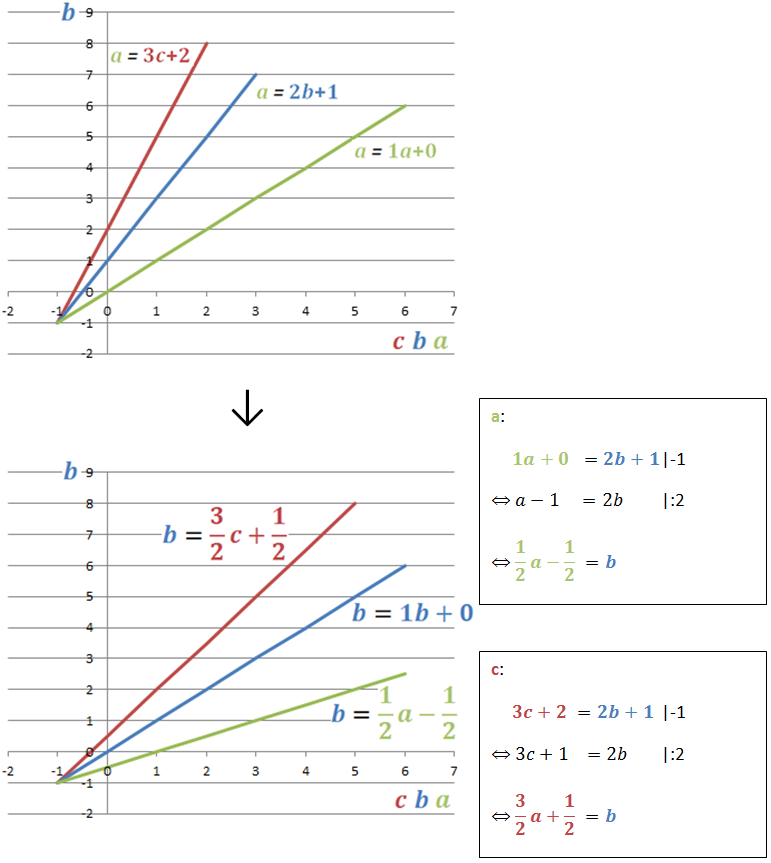
\includegraphics{images/quantity/setDefaultUnit}
	\caption{Umrechnung beim Ändern einer DefaultUnit}
\end{figure}

\subsubsection{Quantitäten} \newline